% !TEX root = C:\Users\Jan\Documents\dev\Risk-Measurement-Framework\masterthesis_tex\masterthesis_main.tex
\section{Evaluation}
\label{sec:evaluation}

A common example to show backdoor attacks is traffic sign detection (\cite{DBLP:journals/corr/abs-2102-10369}, \cite{DBLP:journals/corr/abs-1708-06733}, \cite{DBLP:conf/codaspy/NudingM20},
\cite{DBLP:journals/tdsc/LiXZZZ21}). That makes it easier to find datasets and already finished ML models to make a case study. In the following subsections the focus lies on the case study which concept and its implementation is evaluated here. \\ Further, the requirements and procedures from ISO 27004 in relation with the RMF is discussed in this section. In addition, this section describes real-world examples for which the RMF could be used.

\subsection{Evaluation of the ISO 27004 standard in context to the RMF}

Sections \ref{sec:conFrame} and \ref{sec:implementation} show both that it is possible to design and implement a technical framework for ML security especially risk measurement based on ISO 27004 \cite{ISO_27004_2009}. Also, the decisions that come individually from the organization had to be disregarded by using specific attacks and risk indicators because there is no choice available at this point. However, as soon as individual decisions are required, such as information needs and stakeholder identification, it is no longer possible to implement this without human decisions.

\subsection{Case Study: Developing a SVM for traffic sign detection}

For the case study scikit-learn \cite{scikit-learn} and for preparation of the dataset in Python OpenCV2 have different function to load and resize images \cite{opencv_library}. In their work, Stallkamp et al. \cite{DBLP:conf/ijcnn/StallkampSSI11} built a mulit-category classification dataset. The mulit-category classification dataset contains german traffic signs for image classification. That mulit-category classification dataset uses the german traffic signs from a approx. 10 hours daytime video from different roads.
This case study is an example to show the functions and results of the RMF. After showing this case study there will be explain and discuss realistic case studies where backdoor attacks could have a more realistic impact for scores of ML models.

\subsubsection*{Structure of the ML model for the case study}

The original dataset from Stallkamp et al. \cite{DBLP:conf/ijcnn/StallkampSSI11} is splitted between a training and testing folder. The training folder separate 43 signs into subfolders. This subfolders make it easy to use specific traffic signs which decrease the training time. The information of the folders are written in an eponymous csv-file that are not needed further in this case study. In Figure \ref{fig:traffic_signs} the shown traffic signs can be used for training the SVM and are all labeled in the data preprocessing like the subfolder name 0 - 42. The training set contains traffic signs such as speed limit, prohibitory, derestriction, mandatory, danger, and unique signs.

\begin{figure}[h!]
  \centering
  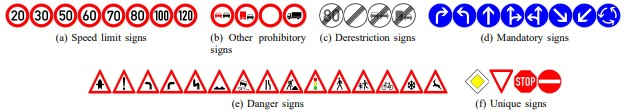
\includegraphics[width=12cm]{pictures/traffic_signs.jpg}
  \caption{Labeled traffic signs adapted from \cite{DBLP:conf/ijcnn/StallkampSSI11}.}
  \label{fig:traffic_signs}
\end{figure}

\begin{figure}[h!]
  \centering
  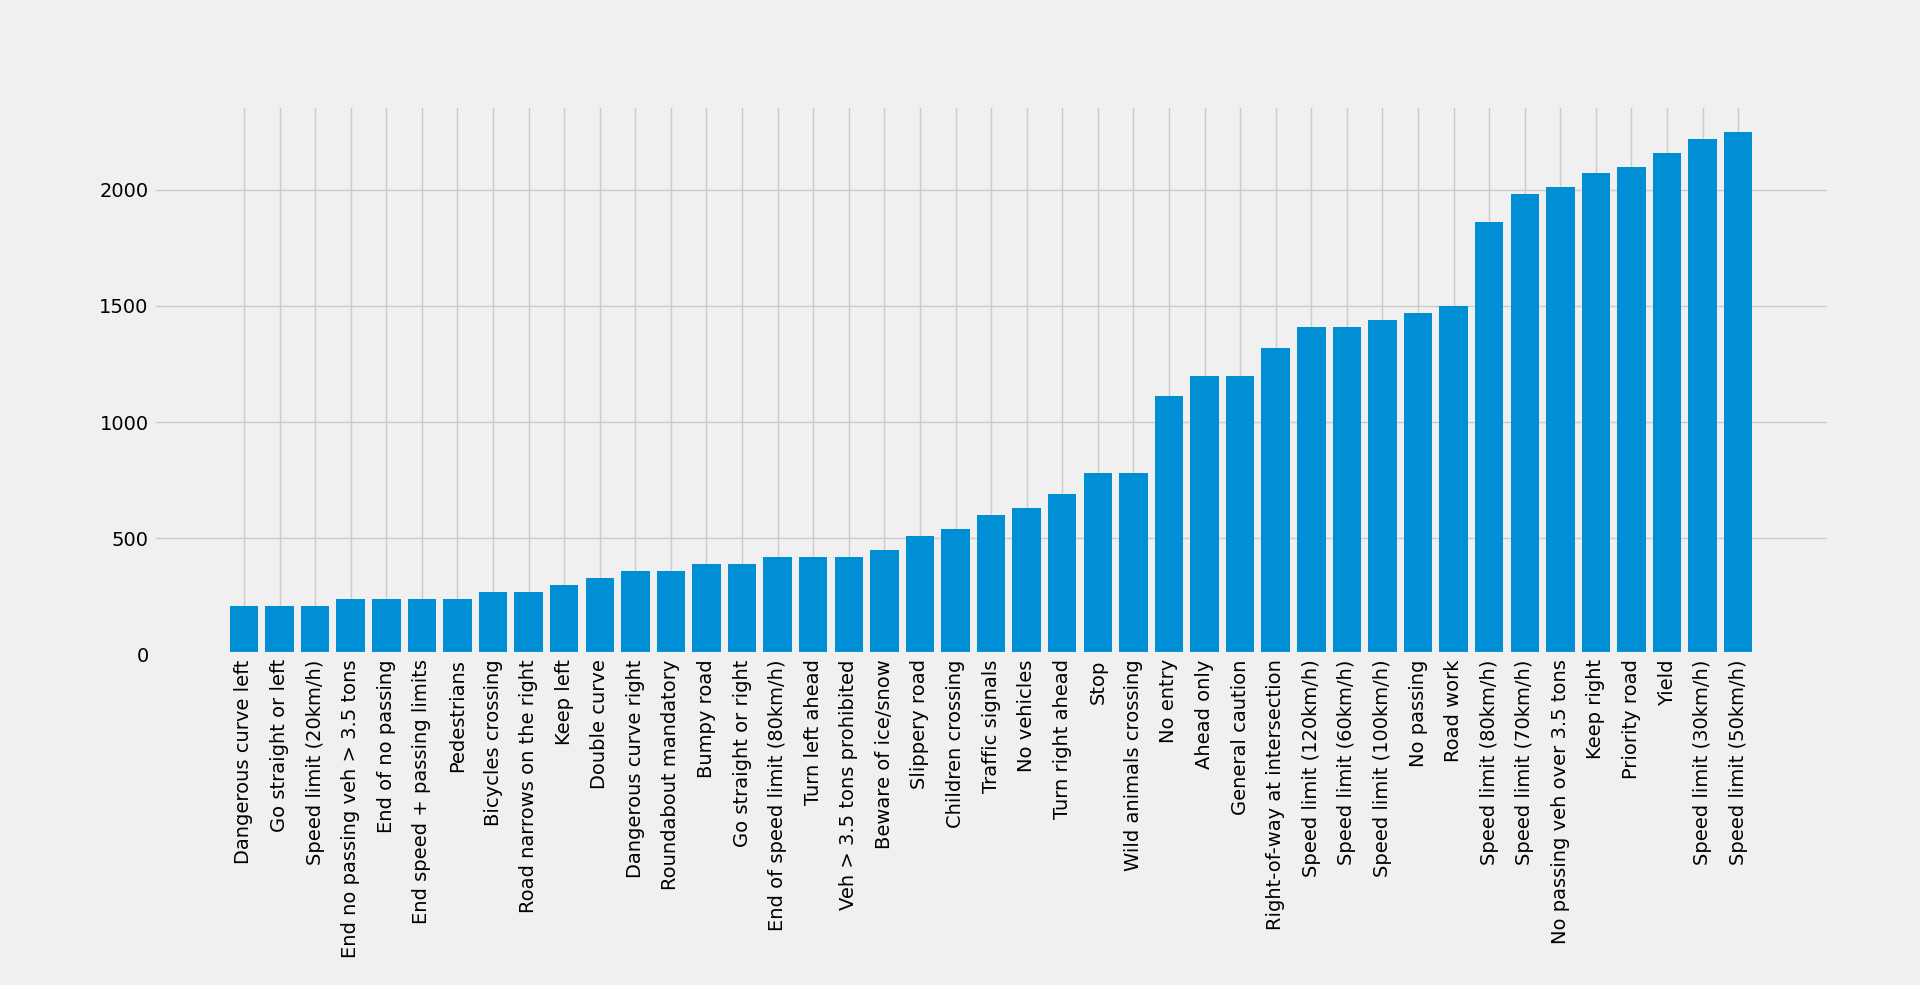
\includegraphics[width=15cm]{pictures/num_of_images.png}
  \caption{Number of images per labels.}
  \label{fig:num_of_images}
\end{figure}

All signs are resized to 50x50 pixel to optimize the performance of the NN. The training sets are also scaled with Keras and TensorFlow to execute the attacks successfully. The training data and test data load from two different folders and are trained during ten epochs. All functions, the arguments and a description of them can be found in appendix \ref{sec:case_study_functions}. Figure \ref{fig:nn} shows the NN architecture.

\begin{figure}[h!]
  \centering
  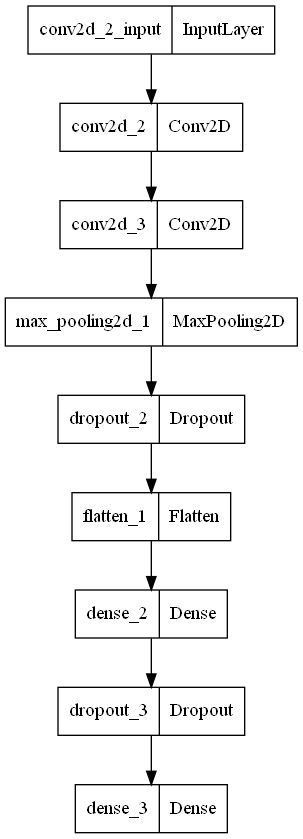
\includegraphics[width=5cm]{pictures/nn.png}
  \caption{Generated NN architecture image from Keras.}
  \label{fig:nn}
\end{figure}

The computer to execute the ML model have resources such as, AMD Ryzen \cite{DBLP:conf/hotchips/AroraBW20} 7 5800X 8-Core Processor with 3.80 GHz, 16 GB of RAM, and a NVIDIA GeForce RTX \cite{DBLP:journals/pcs/SanzharovFG20} 3060 Ti. These resources are available to the attacker and to measure the computational resources to get the attacker's effort.

\subsection{Differences between manipulated and original dataset}

\begin{figure}[ht!]
  \centering
  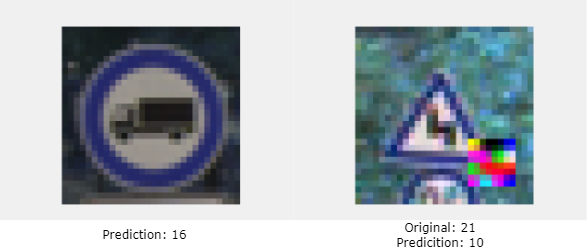
\includegraphics[width=10cm]{pictures/backdoor_example_rmf.png}
  \caption{The left image shows a clean output. The right image shows a poisoned output with a wrong prediction. Both images are the output from the ML model with the \textit{Clean Label Backdoor Attack} from the RMF.}
  \label{fig:backdoor_example_rmf}
\end{figure}

The Python plots from the case study show in this subsection examples images to show the differences between the original and manipulated dataset. Figure \ref{fig:backdoor_example_rmf} visualizes the prediction of the ML model with the attack of the RMF. If the ML model is executed multiple times, the poisoned image show always the same wrong label because the attack specificity is targeted.

\subsection{Results from the measurement methods}

For this case study, the ML model is attacked by a \textit{Clean Label Backdoor Attack} with a backdoor trigger that Figure \ref{fig:poisoned_hidden_trigger} shows. $50\%$ of the images are poisoned during the attack to missclassify to the label \textit{10: No passing veh over 3.5 tons}.

\subsubsection*{Risk indicators to measure the attacker's effort}

\noindent\textbf{Attacker's goal} As the attack is a backdoor attack, the RMF returns for the attacker's goal an inference failure. It takes six steps to develop a backdoor attack. These development steps are generalized and base not on a specific attack. The RMF returned these six steps as a natural number which shows, that the RMF measured the correct goal. \\

\noindent\textbf{Attacker's knowledge} This risk indicator returned the number of steps to implement the \textit{Clean Label Backdoor Attack}. Based on the work of Turner et al. \cite{turner2018clean}, this thesis figured out that it takes ten steps to implement this attack. The ART \cite{art2018} define which information are to be used as parameters to execute this attack. \\

\noindent\textbf{Computational resources} The computational resources that are measured are the CPU, GPU, and RAM. The RAM measurement starts at the beginning of the implemented ML model and shows after finishing the training time of the ML model how much RAM resources the ML model uses. The CPU and GPU are measured directly after the training without a start point. The training time without the attack uses $970.7B$ RAM, $7.2\%$ CPU (which is $0.07$), and $8094.27MB$ of the GPU.\\ The training time with the implemented attack uses $1825.73MB$ RAM, $9\%$ CPU (which is $0.09$), and $8137.81MB$ of the GPU. The CPU and RAM measurement do not measure the training time of the ML model, but from the complete Python program.

\subsubsection*{Risk indicators to measure the extent of damage}

\noindent\textbf{Attack time} All backdoor attacks are executing during training time. Figure \ref{fig:feature_match} shows that FLANN and SIFT found the backdoor in a poisoned image. The time to train a ML model without the attack and inference time takes $962.14$ seconds. When the attack is added, it is $1037.23$ seconds.

\begin{table}[ht!]
\centering
  \begin{tabular}{| l | p{1.5cm} | p{2cm} | p{1.5cm} | p{1.5cm} |}
  \hline
  \rowcolor{lightgray} Label & TP & TN & FP & FN \\ [0.5ex]
  \hline
  Speed limit (20km/h) & 59 & 12570 & 0 & 1 \\
  Speed limit (30km/h) & 707 & 11898 & 12 & 13 \\
  Speed limit (50km/h) & 743 & 11873 & 7 & 7 \\
  Speed limit (60km/h) & 430 & 12169 & 11 & 20 \\
  Speed limit (70km/h) & 655 & 11959 & 11 & 5 \\
  Speed limit (80km/h) & 620 & 11953 & 47 & 10 \\
  End of speed limit (80km/h) & 132 & 12480 & 0 & 18 \\
  Speed limit (100km/h) & 428 & 12175 & 5 & 22 \\
  Speed limit (120km/h) & 431 & 12173 & 7 & 19 \\
  No passing & 479 & 12132 & 18 & 1 \\
  No passing veh over 3.5 tons & 656 & 11968 & 2 & 4 \\
  Right-of-way at intersection & 416 & 12204 & 6 & 4 \\
  Priority road & 682 & 11937 & 3 & 8 \\
  Yield & 718 & 11907 & 3 & 2 \\
  Stop & 269 & 12360 & 0 & 1 \\
  No vehicles & 210 & 12413 & 7 & 0 \\
  Veh > 3.5 tons prohibited & 149 & 12478 & 2 & 1 \\
  No entry & 351 & 12269 & 1 & 9 \\
  General caution & 383 & 12229 & 11 & 7 \\
  Dangerous curve left & 60 & 12562 & 8 & 0 \\
  Dangerous curve right & 89 & 12522 & 18 & 1 \\
  Double curve & 84 & 12538 & 2 & 6 \\
  Bumpy road & 109 & 12509 & 1 & 11 \\
  Slippery road & 144 & 12477 & 3 & 6 \\
  Road narrows on the right & 89 & 12538 & 2 & 1 \\
  Road work & 476 & 12128 & 22 & 4 \\
  Traffic signals & 170 & 12445 & 5 & 10 \\
  Pedestrians & 60 & 12568 & 2 & 0 \\
  Children crossing & 147 & 12478 & 2 & 3 \\
  Bicycles crossing & 87 & 12540 & 0 & 3 \\
  Beware of ice/snow & 133 & 12480 & 0 & 17 \\
  Wild animals crossing & 266 & 12353 & 7 & 4 \\
  End speed + passing limits & 60 & 12568 & 2 & 0\\
  Turn right ahead & 209 & 12417 & 3 & 1 \\
  Turn left ahead & 119 & 12508 & 2 & 1 \\
  Ahead only & 389 & 12236 & 4 & 1 \\
  Go straight or right & 115 & 12508 & 2 & 5 \\
  Go straight or left & 58 & 12569 & 1 & 2 \\
  Keep right & 684 & 11934 & 6 & 6 \\
  Keep left & 88 & 12540 & 0 & 2 \\
  Roundabout mandatory & 87 & 12535 & 5 & 3 \\
  End of no passing & 45 & 12561 & 9 & 15 \\
  End no passing veh > 3.5 tons & 79 & 12534 & 6 & 11 \\
  \hline
  \end{tabular}
  \caption{True and False values (left) before the attack, (right) after the attack.}
  \label{tab:pos_neg}
\end{table}

\noindent\textbf{TP, TN, FP, FN} Table \ref{tab:pos_neg} shows the TP, TN, FP, and FN from the last epoch before and after the attack.

\noindent\textbf{Accuracy} The accuracy is a risk indicator should be decreased as much as possible if an ML model is attacked with a backdoor attack. The original ML model has an accuracy of $0.94$ and the accuracy with the poisoned dataset $0.06$. \\

\noindent\textbf{Attack specificity} The \textit{PoisoningAttackCleanLabelBackdoor} is a targeted attack which means for the attacker it takes four steps to choose a specific label. If there are more than one source and target label then the number of steps would be increased. The following steps must be performed:

\begin{enumerate}
  \item Choosing the label \textit{10: No passing veh over 3.5 tons}
  \item Choose a number of images to poison
  \item Choose the possible labels to poison (all labels)
  \item Selecting the target images randomly to poison
  \item Transmit the selected images to the PGD
\end{enumerate}

\subsection{Evaluation of the measurement construct}

After the measurement methods, the RMF evaluates the base measures. For this purpose, all values must be unified so that they can be added together. This unification works only for the extent of damage because the corresponding risk indicators have values whose units can be adjusted in each case. The TP, TN, FP, FN is a risk indicator that calculates the ML metrics which have the same unit as the accuracy. This relation makes it possible to convert the ML metrics and the accuracy into a standartized unit. In combination with the number of successfully missclassifications which can be also despicted as the same unit as the ML metrics and the accuracy, it is possible to calculate all values with the sum formula to the extent of damage as a total value. \\
The attacker's effort forms from the total number of steps the attacker has to do to execute the attack, the time and the computational resources. These different risk indicators have no approach to be offset by uniform values. Therefore this does not lead to a plausible result, the values can not be combined to a common value, but can be considered individually. From this point on, the measurement construct is adjusted so that all calculated values are presented separately in different risk matrices at the end.

\subsubsection*{Derived measures}

\noindent\textbf{ML metrics} The following Figures show the ML metrics with the original predicitions and the poisoned predicitions during inference time.

\begin{figure}[!tbp]
  \centering
  \begin{minipage}[b]{0.4\textwidth}
    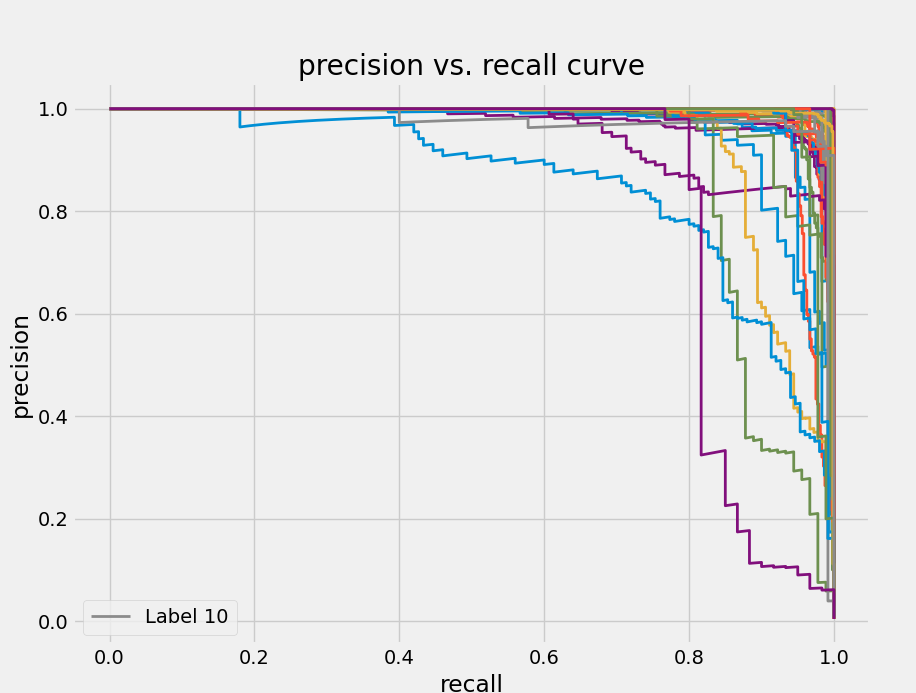
\includegraphics[width=8cm]{pictures/precision_recall_curve.png}
    \caption{The precision-recall curve of the original test dataset. Each color represents a class of the ML model.}
    \label{fig:precision_recall_curve}
  \end{minipage}
  \hfill
  \begin{minipage}[b]{0.4\textwidth}
    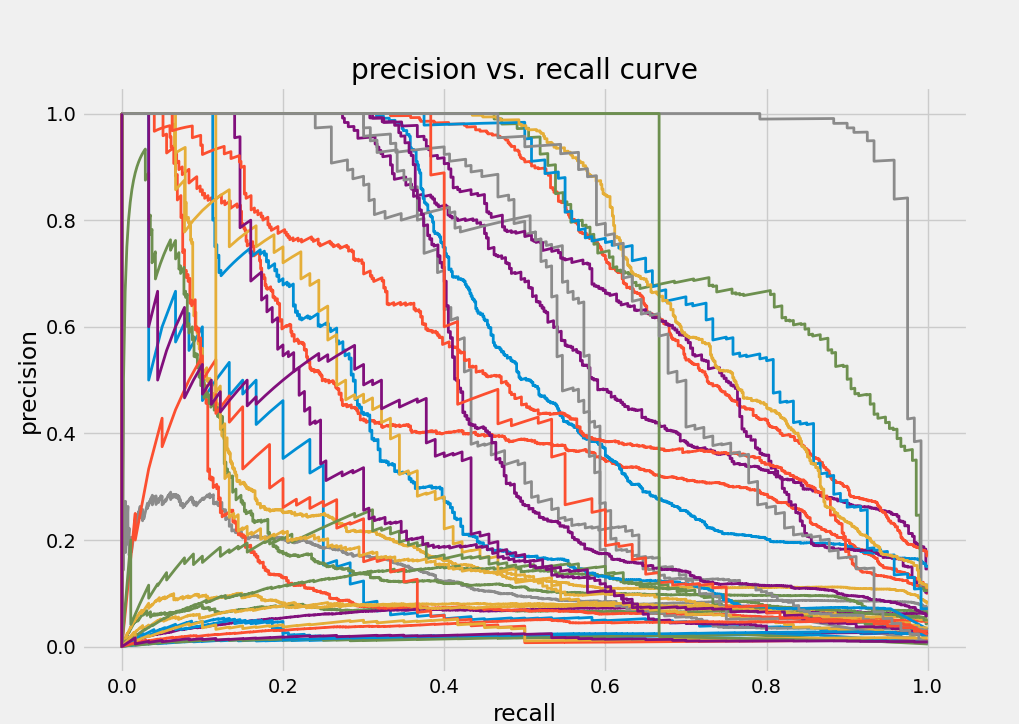
\includegraphics[width=8cm]{pictures/poisoned_precision_recall.png}
    \caption{The precision-recall curve of the poisoned test dataset. Each color represents a class of the ML model.}
    \label{fig:poisoned_precision_recall}
  \end{minipage}
\end{figure}

Figure \ref{fig:precision_recall_curve} and \ref{fig:poisoned_precision_recall} show the different precision-recall curves of the original test dataset and the poisoned dataset. Each colored function represents the progression of a label. Figure \ref{fig:precision_recall_curve} shows a clear tendency of the precision-recall curve where the recall values increase steadily while the precision values decrease that the ML model makes the best accessible distinctions. As a result, the predictions become closer to the actual results, which causes the threshold to further separate the TP and FN values from the FP and TN. \\
Figure \ref{fig:poisoned_precision_recall} shows how the precision-recall curve proceeds after the original test dataset is poisoned with the same poisoning function which is used for the original training dataset. This curve shows that the clear tendency of the process for each label is no longer present except for the target label of the backdoor attack. That tendency shows the effectivness of the attack because there is only the target label which compares to the precision-recall curve of the target label. \\
The only label that hardly changes in Figures \ref{fig:precision_recall_curve} and \ref{fig:poisoned_precision_recall} is label \textit{10: No passing veh over 3.5 tons}, since this was defined as the target label and is still classified as the correct label in the prediction.

\begin{figure}[ht!]
  \centering
  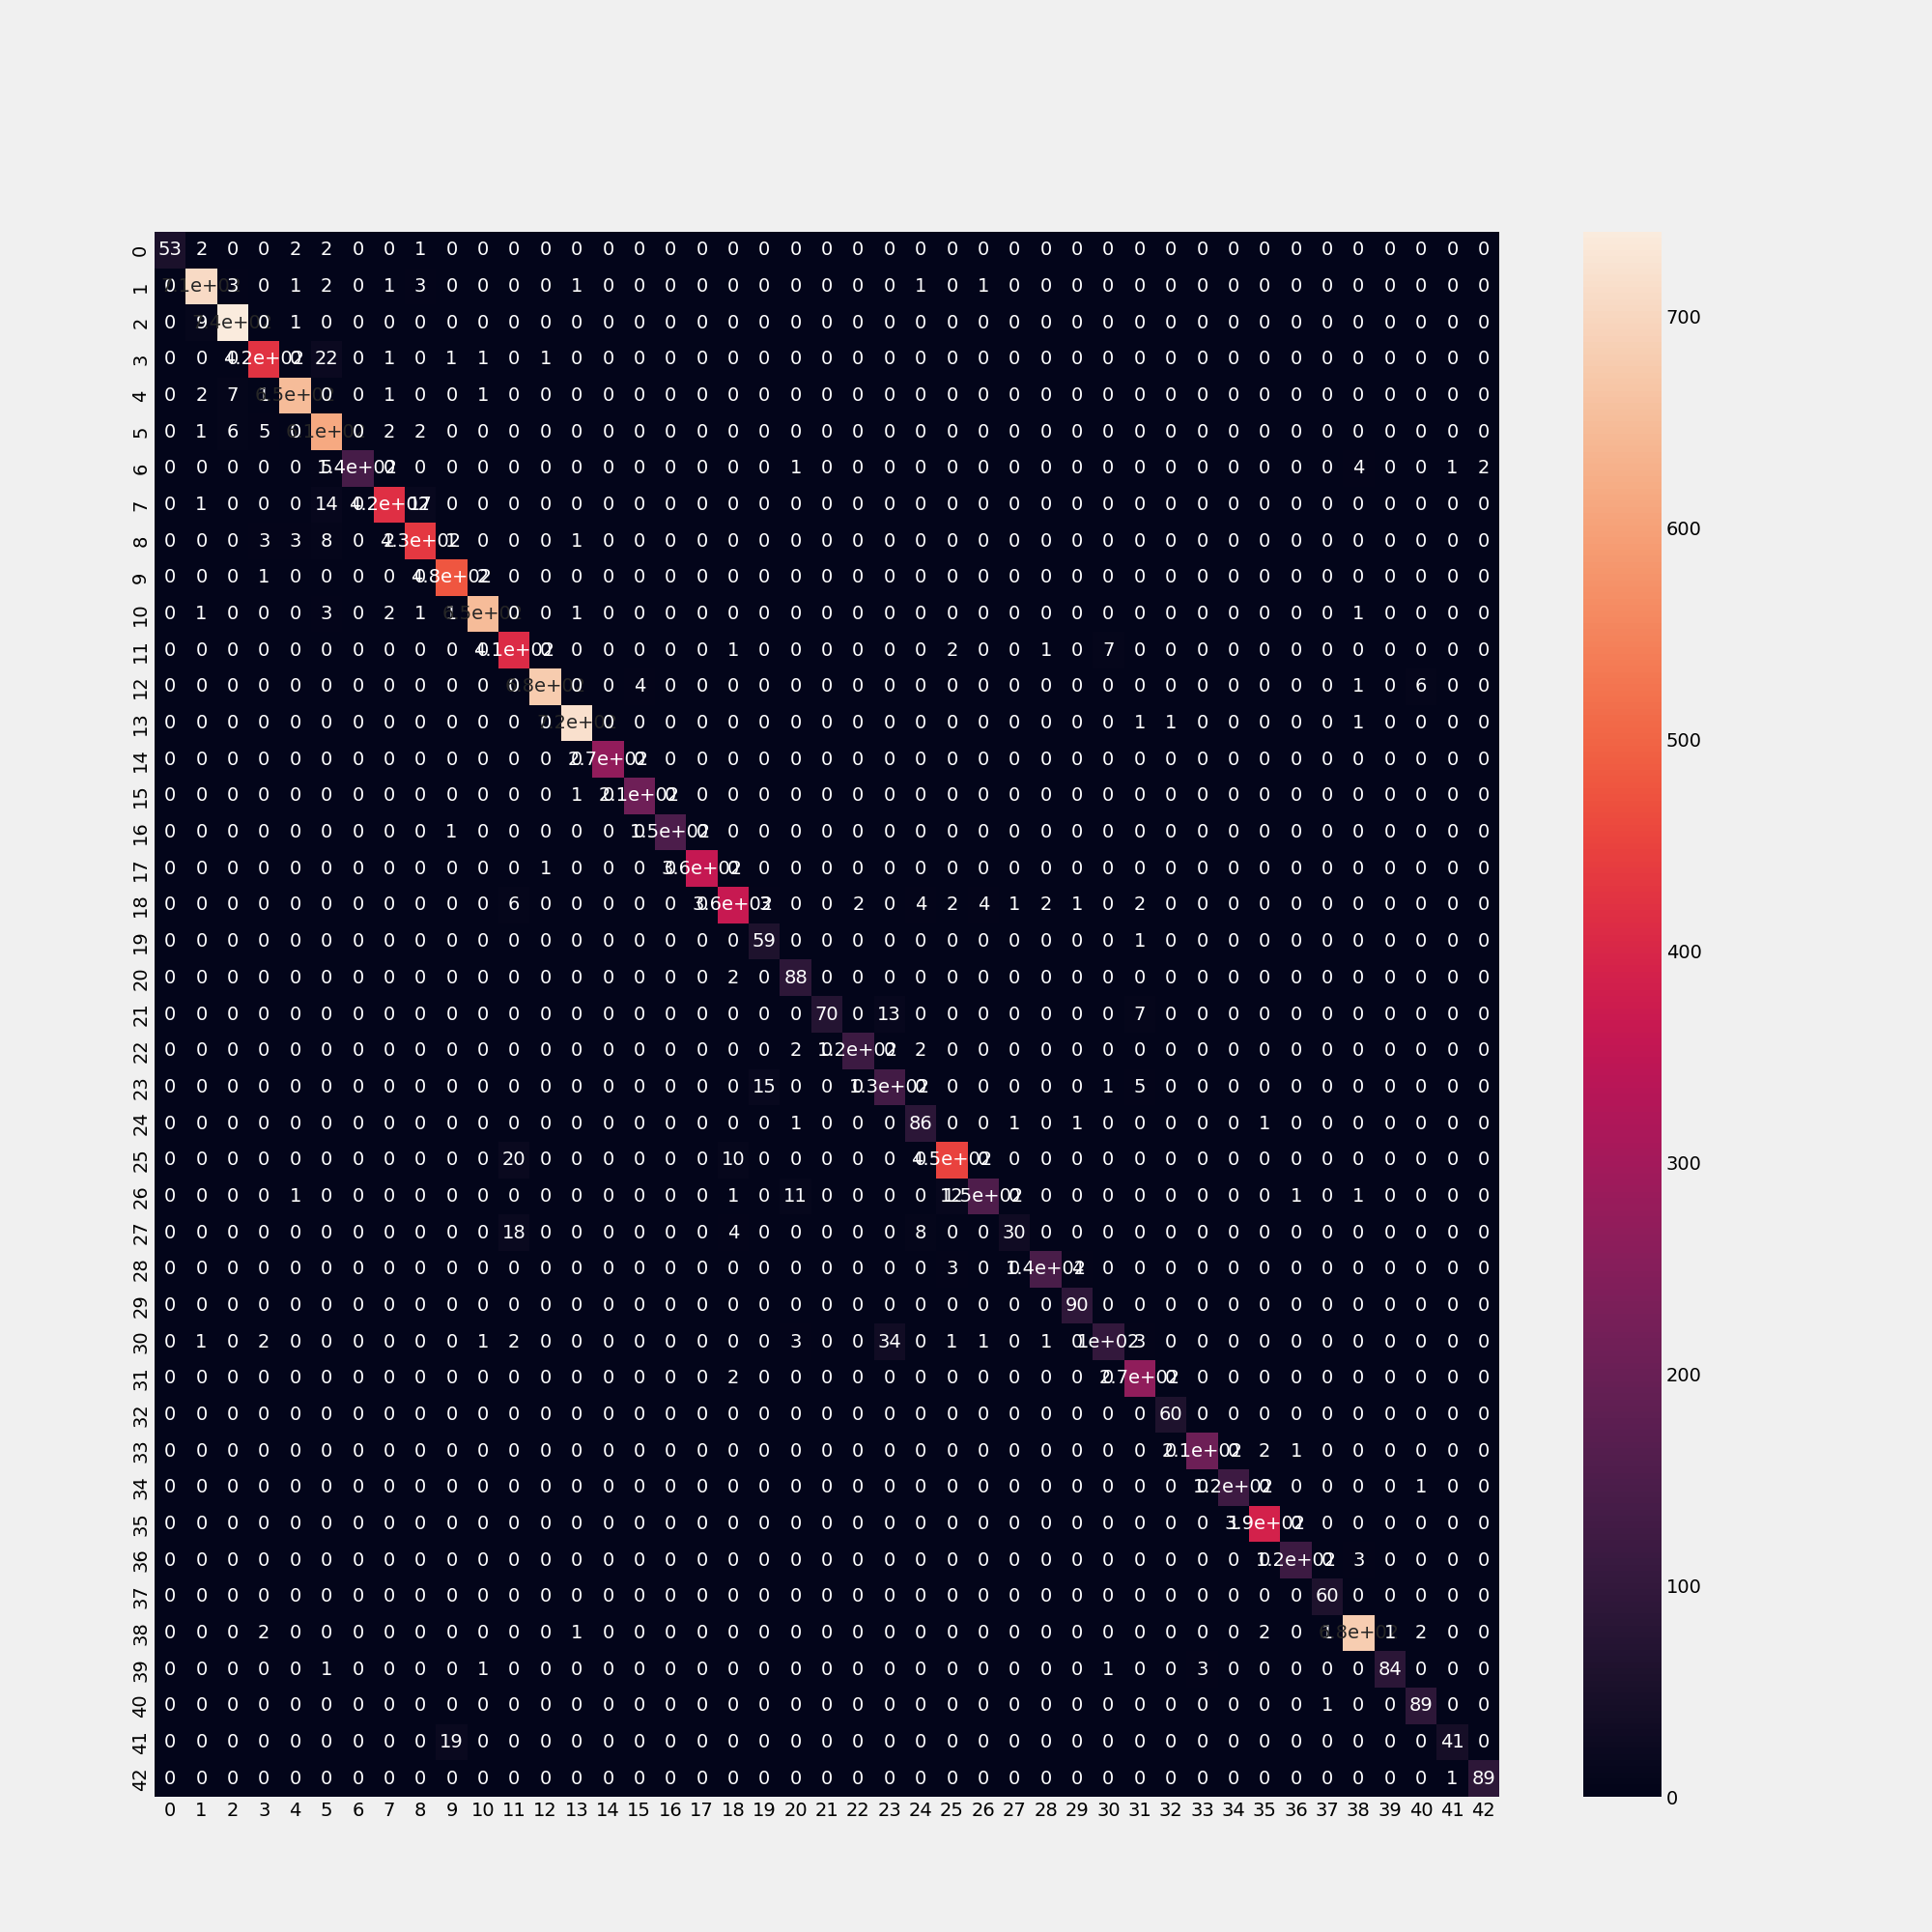
\includegraphics[width=11cm]{pictures/cm_original_testdata.png}
  \caption{The confusion matrix of the original test dataset.}
  \label{fig:cm_original_testdata}
\end{figure}

\begin{figure}[ht!]
  \centering
  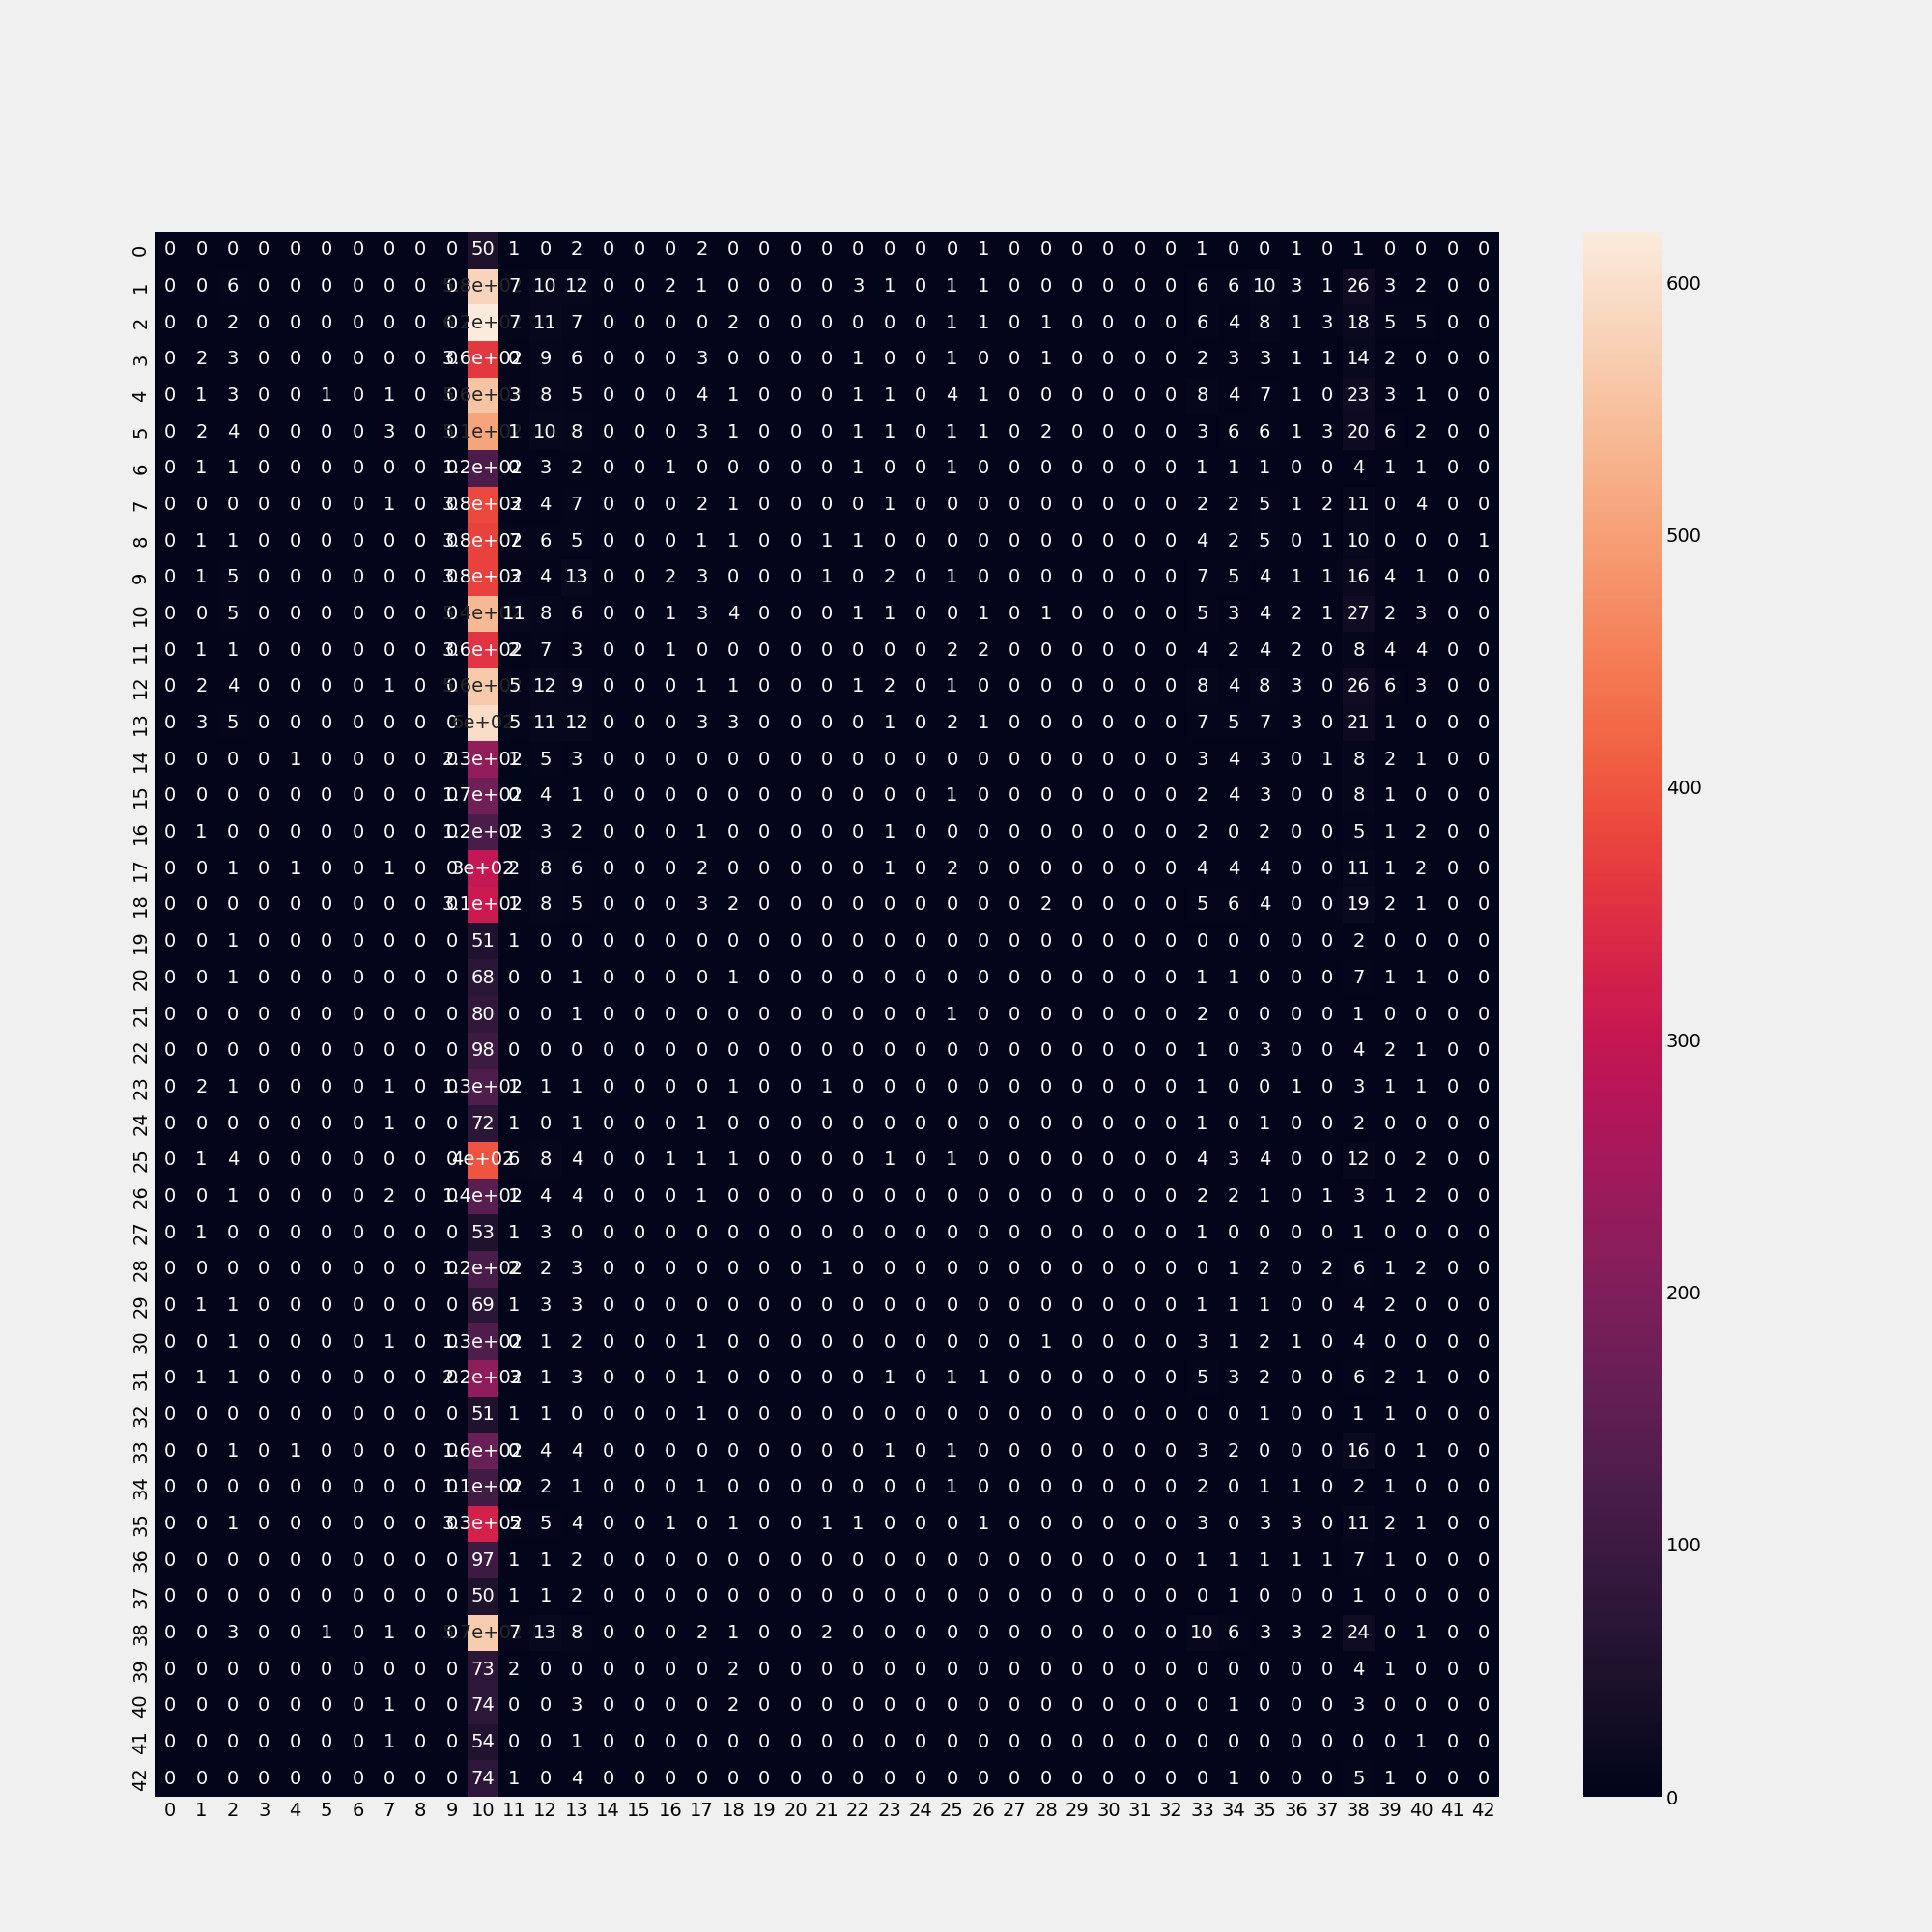
\includegraphics[width=11cm]{pictures/cm_poisoned_testdata.png}
  \caption{The confusion matrix of the poisoned test dataset.}
  \label{fig:cm_poisoned_testdata}
\end{figure}

Figure \ref{fig:cm_original_testdata} and \ref{fig:cm_poisoned_testdata} show the different confusion matrices of the original test dataset and the poisoned dataset. The confusion matrix in Figure \ref{fig:cm_original_testdata} shows the summarized predictions of the original testdata. Each column of the matrix summarizes the predictions and each row the actual labels. Most of the predictions and their actual labels run diagonally in the confusion matrix, as shown by the lighter colors. The brighter an index is, the higher its value. \\
In relation to the confusion matrix in Figure \ref{fig:cm_poisoned_testdata}, the predictions change towards label \textit{10: No passing veh over 3.5 tons}, since this is the target label of the attack. The matrix also shows the actual labels in the darker indices. Therefore, the confusion matrix can also be used to visually depict the difference between the original and the poisoned test dataset. \\
In order to calculate the extent of damage with the ML metrics, the precision, recall, and F1-Score are all calculated for each label and then summarized them as their average value which table \ref{tab:ml_metrics} shows.

\begin{table}[ht!]
  \centering
  \begin{tabular}{| c | c | c |}
  \hline
  \rowcolor{lightgray} ML metric & Original value & Poisoned value \\ [0.5ex]
  \hline
  Average Precision & 0.96 & 0.02 \\
  \hline
  Average Recall & 0.94 & 0.02 \\
  \hline
  Average F1-Score & 0.94 & 0.01 \\
  \hline
  \end{tabular}
  \caption{Average ML metrics value between the original and the poisoned test dataset.}
  \label{tab:ml_metrics}
\end{table}

\noindent\textbf{Derived damage values} After calculating the ML metrics, this measurement function calculate based on the attack time and specificity how many images are missclassified successfully and count the number of these images. The function count the number of target labels. It is important that, as mentioned above, the poisoned dataset only takes images that do not already have the target label. These would otherwise falsify the result. After the comparing is finished, then this function gets the number of possible poisoned images from the attack specificity and calculates the result as the percentage value to unify the result with the other values for the extent of damage. \\
The reversed value of the accuracy is $9.94$, average precision is $9.98$, average recall is $9.98$, and the average F1-Score $9.99$, the total number of poisoned images is $ $ which are $ $ and as a decimal value $ $. This number do not has to be reversed because if the number of images decreases, then the decimal value decreases which would lower the extent of damage.

\noindent\textbf{Derived attack steps} The attack steps calculate from the attacker's knowledge, attacker's goal, and attack specificity. At this point, the attack time is no longer considered but is passed to the analytical model as a separate value. \\
After calculating all steps together, the attacker has to perform 21 steps to achieve the inference failure, implement and execute the \textit{PoisoningAttackCleanLabelBackdoor}, and poisoning a random amount of all labels to missclassify images to the target label \textit{10: No passing veh over 3.5 tons}.

\noindent\textbf{Analytical models} This step in the RMF should calculate the base and derived measures originally into the extent of damage and the probability of occurrence. The extent of damage can still be calculated but the probability of occurrence cannot. The extent of damage is calculated by the reversed accuracy and average ML metrics to increase or decrease the damage the closer or further away the accuracy and the average ML metrics are.

\subsection{The decision criteria and measurement results}

\subsection{Poisoning and backdoor attacks in real applications}

Beside the exemplary application from the case study, the scientific papers in this subsection show real applications where the RMF can then help in a more real environment. An example for real-world poisoning attacks against ML models is Microsoft's chatbot Tay. This chatbot learned racist and offensive language from Twitter users \cite{DBLP:conf/iciot/BaracaldoCLSZ18}, \cite{DBLP:conf/ccs/BaracaldoCLS17}. Microsoft removed the bot after 16 hours because the bot produced offensive tweets.
